\chapter{Attack Simulation}
\label{cap:attacksimulations}

% ES-CMA reliability based

\section{Detection of Unstable Challenges}

For the reliability based \ac{ES-CMA} attack on \apufs it is crucial to find challenges which evaluate differently at multiple evaluations as explained in Sec. \ref{sec:cma-es}.
To find these challenges and their reliability $\gls{h}$ every challenge $\gls{c}$ of a set will be evaluated $\gls{j}$ times.
After that the reliability $\gls{h}$ will be computed for every challenge by \ref{equ:reliability}.
When using \ac{MV} to increase the stability of the \apuf finding challenges with lower reliability becomes more difficult.
Hence Fig. \ref{fig:cmamajorityvotemeasurementrelation} shows the relation between the increase of votes $\gls{m}$ and the decrease of found challenges which lowered reliability $\gls{h}$.
In this case a lowered reliability is already reached if a challenge $\gls{c}$ evaluates one or multiple times different to the rest of the evaluations for $\gls{j}$ number of evaluations and is called unreliable.
There are four line graphs for the different $\gls{j}$ number of evaluations.
The lowering gradient of all four graphs display the subsiding impact of \ac{MV} with rising $\gls{m}$ as explained in Sec. \ref{sec:stabilityimprovementbymajorityvote}.
The little difference between the graphs shows that increasing the number of evaluation $\gls{j}$ does not necessarily provides more challenges with lowered reliability $\gls{h}$.
Without \ac{MV} there is a little increase of found challenges with lowered reliability $\gls{h}$.
Though with applying \ac{MV} this increase disappears with growing $\gls{m}$.

\begin{figure}[ht]
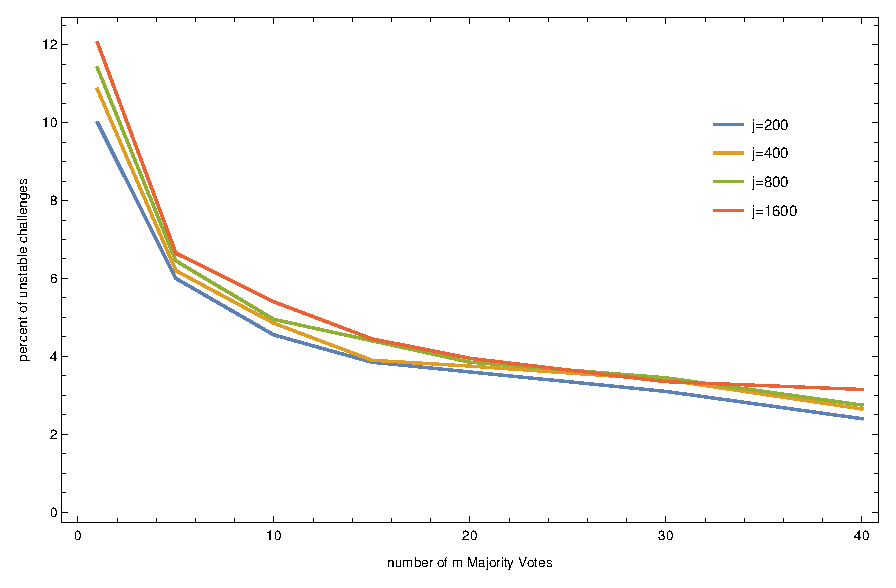
\includegraphics[width=1.00\textwidth]{images/mv-measurements-unstableChallenges.eps}
% \noindent\includegraphics[width=1.00\textwidth, height=3cm, draft]{example-image-a}
\caption{Proportion of unreliable challenges for different values of $\gls{m}$ \ac{MV} votes. The different line graphs represent the $\gls{j}$ number of evaluations $200, 400, 800, 1600$. The small distance between the graphs in the beginning show the very little increase of found unreliable challenges and how this gap resolves with introducing of \ac{MV}.}
\label{fig:cmamajorityvotemeasurementrelation}
\end{figure}

% mv vs. measurements
% unstable challenges are required for the cma-es attack
% Finding unstable challenges: graph!
%========================================

\section{\apufs vs. \mpufs}

$\gls{n} = 32$
$\gls{j} = 100$

training set $10000$
test set $10000$

exit criteria sigma = 0.2

avg on all successful performed attacks where the test set min. 0.8 correct


%========================================

\section{\acs{XOR} \apufs vs. Majority \acs{XOR} \apufs}



\xpuf to unstable with growing k




%========================================

